\chapter{Coreference resolution using rules and domain-dependent features}
\label{chapter:Coreference resolution using rules and domain-dependent features}
\section{Overview}

In this chapter, I will describe the implementation of a new method in protein coreference resolution. I used corpus based rules to deal with problem of pronominal coreference resolution. 

The corpus consists of  research papers' abstracts, thus, I can assume that the text is written in formal way and authors followed syntax rules. From this hypothesis, I got an idea to  generate syntax rules that model relationship between clauses' subjects  in sentence. 

For definite noun coreference resolution, I use domain dependent features, rules and semantic classification. Also, I realised that the order of the rules influences the accuracy of the system, thus, I defined an order of rules, which I applied on definite noun coreference resolution. This new method effects the result by improving both the recall and precision of the system. 

To build the system, I used the paradigm "divide and conquer". Each type of anaphoric expression is resolved in different way based on its syntax role in the sentence structure. I divided the anaphoric expressions in two main types: pronominal anaphoric expressions and definite noun (phrase) anaphoric expressions. 

Because pronouns can have different role in the sentence, I divided  pronouns into three classes:

\begin{itemize}
	\item relative pronouns: that, which, whom and whose 
	\item personal pronouns: it and they 
	\item possessive pronouns:its and their
\end{itemize}

To extract these rules, I used the training data set of the BioNLP corpus. First, I generated different statistics of the corpus and calculated the distribution of anaphoric expressions, antecedents and coreference links. 

I used the statistics to get knowledge about the corpus and they led me to research following characteristics of the corpus:

\begin{itemize}
	\item the structure of the training data set via mining
	\item patterns 
	\item structure of the language used in the articles
	\item deeper statistics on anaphors, antecedents and their relationship
	\item clauses relationship in the sentence
	\item anaphora's role in the sentence
	\item syntactic rules
	\item window size of the search space
\end{itemize}

\section{Data set}

As I have described in the first chapter, I have used the training set of BioNLP corpus to derive the rules. I have tested the accuracy of the algorithm in the test set and in the corpus of 8 full text documents that I have annotated in a format similar to the BioNLP corpus. I have annotated this corpus of 8 documents on the www.tagtog.net [67,68], which is a web application tool for annotation. I have compared my algorithm with current state of the art algorithms in the development and the test set of BioNLP corpus.

\section{Coreference resolution system architecture}

Coreference resolution systems have a pipeline architecture. My protein coreference resolution system I developed in Java and  published as an open source tool.\footnote{https://github.com/kujta1/CoreferenceResolution}
\newpage
\begin{figure}[t]
	\begin{center}
		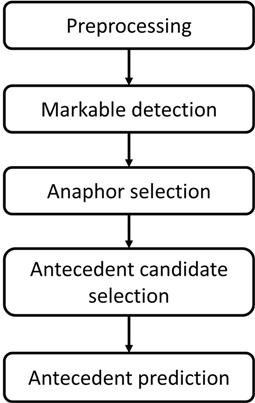
\includegraphics[scale=0.8]{architecture.png} 
 		\caption[Architecture of the coreference resolution system]{ Architecture of the system. As input the system receives two files, the protein annotation file and the text file. The protein annotation file should follow the BioNLP annotation schema. The system after the fifth step, antecedent prediction, will create a file  in which the system will write the coreference links of the inputted text file  [3] }
		\label{Figure 8}
	\end{center}
\end{figure}

The first step is the preprocessing step where the text is dived into sentences. Then, I select all nun phrases the are potential antecedents of an anaphoric expression. In the next step, I select potential antecedent candidates. When  all anaphoric expressions  are selected then for each anaphoric expression I select its potential antecedents. In the final step, I select the most likely antecedent candidate for each anaphoric expression.   
   
In the following sections, I will describe the 5 components of my coreference resolution system. 
  
\begin{table}
   \begin{tabular}{ m{20mm} m{113mm} } 
	\footnotesize{Input (PMID - 7964516)}&\footnotesize{T cell hybridomas respond to activation signals by undergoing apoptotic cell death, and this is likely to represent comparable events related to tolerance induction in immature and mature T cells in vivo. Previous studies using antisense oligonucleotides implicated the c-Myc protein in the phenomenon of activation-induced apoptosis. This role for c-Myc in apoptosis is now confirmed in studies using a dominant negative form of its heterodimeric binding partner, Max, which we show here inhibits activation-induced apoptosis.}\\
	\hline
	\footnotesize{Preprocessing of sentence S3}&\footnotesize{S1: T cell hybridomas respond to activation signals by undergoing apoptotic cell death, and this is likely to represent comparable events related to tolerance induction in immature and mature T cells in vivo. S2: Previous studies using antisense oligonucleotides implicated the c-Myc protein in the phenomenon of activation-induced apoptosis. S3: This role] for c-Myc in apoptosis is now confirmed in studies using a dominant negative form of its heterodimeric binding partner, Max, which we show here inhibits activation-induced apoptosis.}\\
	\hline
	\footnotesize{Markable detection} &\footnotesize{S1: \textit{[T cell hybridomas]} respond to \textit{[activation signals]} by undergoing \textit{[apoptotic cell death]}, and this is likely to represent\textit{ [comparable events related to tolerance induction]} in \textit{[immature and mature T cells [in vivo]]}. S2: [Previous studies using\textit{ [antisense oligonucleotides]}] implicated\textit{ [the c-Myc protein]} in \textit{[the phenomenon of [activation-induced apoptosis]]}. S3: \textit{[This role for [c-Myc] in [apoptosis]]} is now confirmed in \textit{[studies]} using a \textit{[dominant negative form of [[its] heterodimeric binding partner,[Max]]]}, \textit{[which] [we]} show here inhibits \textit{[activation-induced apoptosis]}.}\\
	\hline
	\footnotesize{Anaphora selection} & \footnotesize{S1: T cell hybridomas respond to activation signals by undergoing apoptotic cell death, and \textbf{[this]} is likely to represent comparable events related to tolerance induction in immature and mature T cells in vivo. S2: Previous studies using antisense oligonucleotides implicated the c-Myc protein in the phenomenon of activation-induced apoptosis. S3: This role for c-Myc in apoptosis is now confirmed in studies using a dominant negative form of \textbf{[its]} heterodimeric binding partner, Max,[this] we show here inhibits activation-induced apoptosis.}\\
	\hline
	\footnotesize{Antecedent candidate selection and antecedent}& \footnotesize{S1: [T cell hybridomas] respond to [activation signals] by undergoing [apoptotic cell death], and this is likely to represent [comparable events related to tolerance induction] in [immature and mature T cells [in vivo]]. S2: [Previous studies using [antisense oligonucleotides]] implicated [the c-Myc protein] in [the phenomenon of [activation-induced apoptosis]]. S3: \textcolor{red}{[This role for [c-Myc] in [apoptosis]]} is now confirmed in [studies] using [a dominant negative form of \textcolor{blue}{\textbf{\textit{[its]}}} heterodimeric binding partner, Max], which we show here inhibits activation-induced apoptosis.}\\
	\hline
	\footnotesize{Predict antecedent}&\footnotesize{S1: T cell hybridomas respond to activation signals by undergoing apoptotic cell death, and this is likely to represent comparable events related to tolerance induction in immature and mature T cells in vivo. S2: Previous studies using antisense oligonucleotides implicated the c-Myc protein in the phenomenon of activation-induced apoptosis. S3: This role for \textcolor{red}{\emph{\textbf{[c-Myc]}}} in apoptosis is now confirmed in studies using a dominant negative form of \textcolor{blue}{\emph{\textbf{[its]}}} heterodimeric binding partner, Max, which we show here inhibits activation-induced apoptosis.}
  \end{tabular}
  \caption[A simulation of the protein coreference resolution system]{A simulation of the protein coreference resolution system workflow (the text adopted from [3])}
\end{table}

\newpage
\section{Preprocessing}

In this step, I have used sentence segmentation and syntax parsers to structure the inputted text. For sentence segmentation I used Genia sentence splitter and for sentence (deep) parsing I used Enju parser.[50,54]

\section{Markable detection}

After the preprocessing step I knew the structure of each sentence, I selected text chunks that are candidate coreferential expressions. In the MUC-7 jargon, these text chunks are called markables. Noun phrases and pronouns were considered as markables. To reduce the redundant information in markables, I filtered noun phrases that shared the same head word and I selected as potential candidate just the longest noun phrase (Figure 4.2). 

\begin{figure}[h]
	\begin{center}
		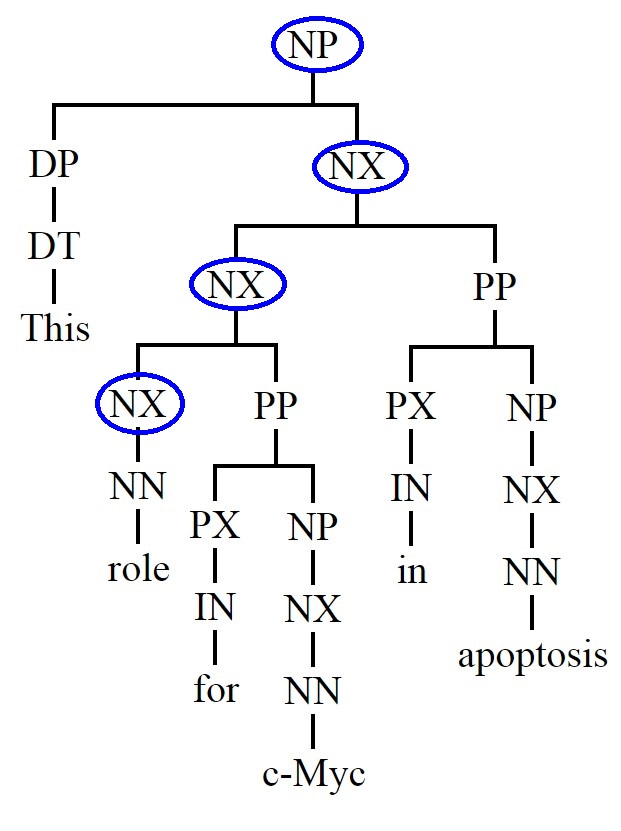
\includegraphics[scale=0.4]{SameHeadWord.jpg} 
 		\caption[Filtering out noun phrases that share the same head word]{ Filtering out noun phrases that share the same head word. In this example, all four noun phrases have the same headword \emph{"role"}. I considered as potential candidate just the longest noun phrases \emph{"This role for c-Myc in apoptosis"}.(In the Enju parser noun phrases are marked with abbreviations NP and NX) }
		\label{Figure 9}
	\end{center}
\end{figure}

Additionally, I did not consider as markables noun phrases that have a subordinate clause in their content (Figure 10).

\begin{figure}[h]
	\begin{center}
		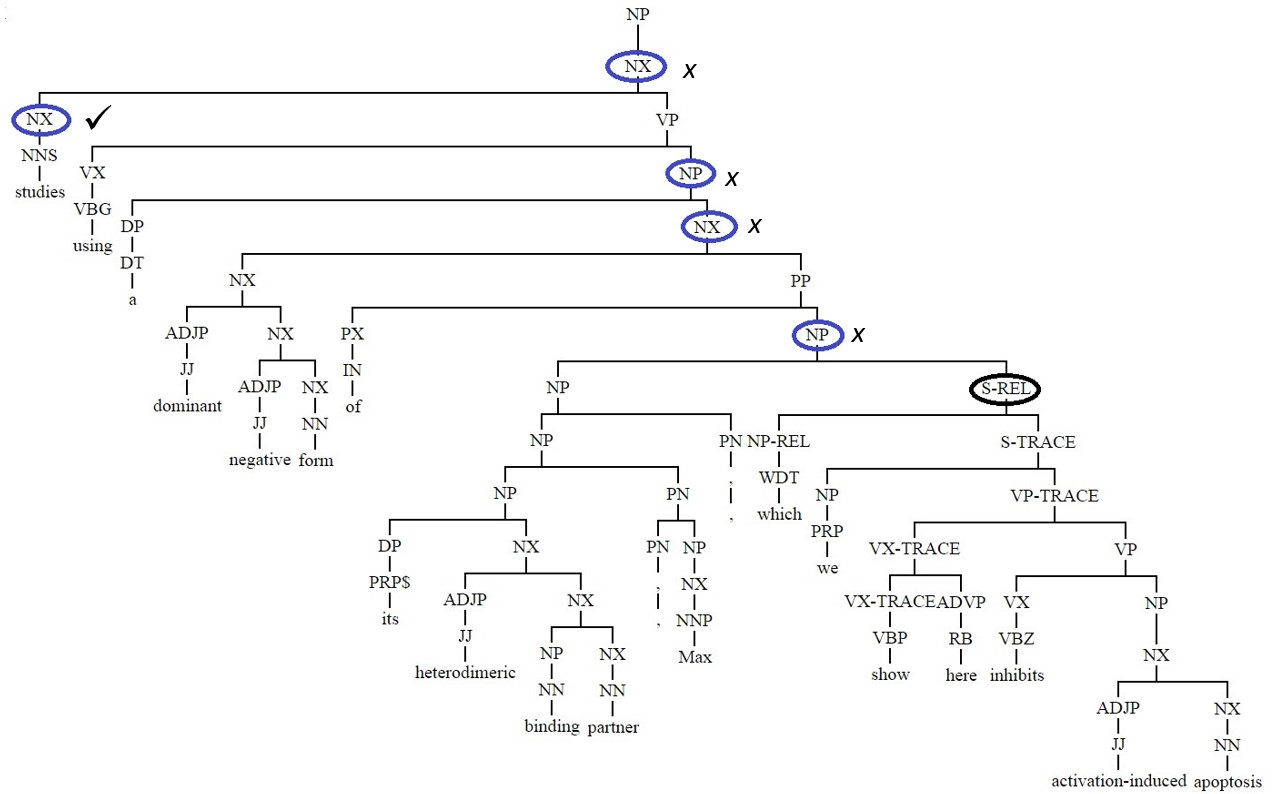
\includegraphics[scale=0.45]{removeSubordinateClause.jpg} 
 		\caption[Filtering out noun phrases that have a subordinate clause in their content]{ Filtering out noun phrases that have a subordinate clause in their content. In this example, I removed noun phrases (marked with \emph{\textbf{x}}) that in their content have the subordinate clause  \emph{"which we show here inhibits activation-induced apoptosis"} }
		\label{Figure 10}
	\end{center}
\end{figure}

\section{Anaphora selection}

\textbf{Anaphora selection} is the step in which I selected text parts that are anaphoric expressions (pronouns and definite noun phrases).
 
I selected the following types of pronouns:

\begin{itemize}
	\item relative pronouns (who, whom, whose, which and that)
	\item personal pronouns (it, they and them)
	\item possessive pronouns (its and their)
	\item definite noun phrases that refer to protein 
\end{itemize}

From the personal pronouns, I just selected the pronouns \emph{"it"} and \emph{"they"} as anaphoric expressions. Other personal pronouns (\emph{I,you,he,she, we and you}) cannot refer to proteins, thus, I filtered and did not select them as anaphoric expressions. Another case of filtering is when the pronoun \emph{"it"} did not refer to any object, for example \emph{"It is important for people to live healthily"}. When the pronoun \emph{"it"} does not refer to an object, it is called \emph{pleonastic}\footnote{ pleonastic (etymology: from Greek word pleonasm which means much, too much) is the phenomena when we use more words than necessary to express a statement to express an idea} \emph{it}. I used patterns to filter pleonastic mentions of the pronoun \emph{it} in similar way like in [3,69]. 

I used these patterns to identify pleonastic it:

\begin{itemize}
	\item \emph{It be $[Adj | Adv | verb]$* that}
	\item \emph{It be Adj $[for NP]$ to VP}
	\item \emph{It $[seems | appears | means | follows]$ that} 
	\item \emph{It has been shown}
\end{itemize}

From possessive pronouns, I only selected the pronouns \emph{its} and \emph{their} as anaphoric expressions. Other possessive pronouns \emph{(my, mine, our, ours, his, her, hers, your, yours)} cannot refer to proteins, thus, I filtered and did not select them as anaphoric expressions.

Identifying anaphoric definite nouns, is a difficult task, because we do not know if a noun phrase is anaphoric or not. In the biomedical domain, many definite nouns do not have an antecedent as the referenced concepts refer to a biomedical entity which is not introduced before or to a general concept. These non-anaphoric expressions appear in scientific texts, because authors assume that the reader has some knowledge in the domain and the authors use the definite noun phrases when they refer to a biomedical entity [3,69]. 

To select the potential anaphoric definite noun phrases, I used semantic knowledge [3,70] and  rules which were generated from the statistics of the corpus. I selected as anaphoric expressions only noun phrases that satisfied the following conditions :

\begin{itemize}
	\item their head noun was protein(s) or gene(s) and start with the words: the, this and these. For example the protein, these two genes and this protein.
	\item their head noun was factor(s), molecule(s), element(s), family, inhibitor(s), receptor(s), complex, construct(s). 
\end{itemize}

Using these filters I covered more than 85\% of the coreference links in the training and the development set.

Indefinite pronouns can act as anaphoric expressions. These cases are not so evident in the biomedical domain. Although these types of expressions are very difficult to identify and my system does not process or try to find these types of anaphoric expressions. In Example 11 the expression "a protein" is an anaphoric expression and its antecedent is "P53". \\
\newpage
\emph{Example (11):}
\begin{changemargin}{10mm}{10mm} 
  \emph{P53, a protein that in humans is encoded by the TP53 gene.}  
\end{changemargin} 
\vspace{4mm}

\subsection{Distribution of anaphoric expressions}
\begin{table}[h]
   \begin{center}
	 \begin{tabular}{|l | C{2cm} C{2cm} C{2cm} C{2cm}|}
 		\hline
  		& BioNLP training data set & BioNLP development data set & BioNLP test data set &Full text data set\\
 		\hline
 		Relative pronouns & 32\% & 34\% & 26\% & 30\% \\
 		\hline 
 		Personal pronouns & 10\% & 12\% & 8\% &12\% \\
 		\hline   
 		Possessive pronouns & 26\% & 29\% & 31\% &19\% \\
 		\hline  
 		Definite noun phrases & 25\% & 19\% & 24\% & 31\% \\
 		\hline  
 		Other & 7\% & 6\% & 11\% &8\% \\
 		\hline   
	\end{tabular}
  \end{center} 
  \caption{ Distribution of anaphoric expressions that refer to protein by  syntactic category}
\end{table}
  
From Table 4.2, we can see that in \emph{the full text data set} the anaphoric definite noun phrases occurs more often than in abstracts. On the other hand, possessive pronouns occur more often in abstracts than in full text.

\section{Antecedent candidate selection}

In my system, I used rules to resolve pronominal anaphora, rules and  domain dependent features to select the antecedent candidate of a definite noun anaphoric expression. These rules I derived based on the assumption that the subjects of clauses in a complex or a compound sentence  refer to the same object,  and two coordinated noun phrases refer to the same object. To select antecedent candidates for definite noun phrases, I used syntactic structure of the sentences and domain dependant features. Most scientists use the nearest candidate to resolve definite noun anaphoric expressions and also claim that the nearest candidate approach is better than best candidate. In my system I implemented a hybrid approach of nearest first and best first [2,4].

\subsection{Statistics of the data sets}
The first step in antecedent candidates selection of  anaphoric expressions was to find a relationship between antecedents and anaphoras. I measured the distance between an anaphoric expressions and their antecedent. This distance, I measured in sentences as  I wanted to know where to look the antecedent of an anaphoric expression.
 
\begin{table}[h]
   \begin{center}
 	  \begin{tabular}{|l | C{2cm} C{2cm} C{2cm} C{2cm}|}
 		\hline
 		& \multicolumn{4}{|c|}{Test set}\\[1.5ex]
 		\hline
 		& D=0 & D=1 & D=2 & D$>$2\\
 		\hline
 		Relative pronouns & 100\% & 0\% & 0\% &0\% \\
 		\hline 
 		Personal pronouns & 80\% & 20\% & 0\% &0\% \\
 		\hline   
 		Possessive pronouns & 83\% & 11\% & 5\% &1\% \\
 		\hline  
 		Definite noun phrases & 31\% & 46\% & 8\% &15\% \\
 		\hline  
 		Other & 47\% & 29\% & 15\% &9\% \\
 		\hline  
  		Total & 72\% & 19\% & 4\% &5\% \\
 		\hline  
     \end{tabular}
   \end{center} 
   \caption{Distribution of anaphoric expressions that refer to protein by category in the \textbf{test set}}
\end{table}

\begin{table}[h]
  \begin{center}
	\begin{tabular}{|l | C{2cm} C{2cm} C{2cm} C{2cm}|}
 		\hline
 		& \multicolumn{4}{|c|}{Test set}\\[1.5ex]
 		\hline
 		& D=0 & D=1 & D=2 & D$>$2\\
 		\hline
 		Relative pronouns & 100\% & 0\% & 0\% &0\% \\
 		\hline 
 		Personal pronouns & 84\% & 16\% & 0\% &0\% \\
 		\hline   
 		Possessive pronouns & 90\% & 10\% & 0\% &0\% \\
 		\hline  
 		Definite noun phrases & 42\% & 34\% & 0\% & 8\% \\
 		\hline  
 		Other & 72\% & 14\% & 14\% &14\% \\
 		\hline  
  		Total & 82.6\% & 12.4\% & 1\% &4\% \\
 		\hline  
	\end{tabular}
  \end{center}
  \caption{Distribution of anaphoric expressions that refer to protein by category in the \textbf{development set}}
\end{table}

From these statistics, I decided to use "divide and conquer" techniques to generate the rules and the window size of the search space for each of 4 types (relative pronouns, personal pronouns, possessive pronouns and definite pronouns) of anaphoric expressions.
And the search space for each type is following: 

\begin{itemize}
	\item relative pronouns - window size of one sentence 
	\item personal and possessive pronouns - window size of two sentences
	\item definite nouns window size of three sentences
\end{itemize}

\subsection{Syntax structure of data set}
From the definition of syntax in section 2.2, we saw that syntax is a set of rules and words. This was a good signal that I could use syntax rules to build a coreference resolution system. An important rule from syntax is that anaphora and antecedent should correspond to their number (singular or plural)\footnote{In other domains is important that the antecedent and anaphora to not have different genders.}. 

The Subject-Verb-Object (SVO) structure of declarative sentences in the English language is the most important rule in coreference resolution. This structure can be defined as: "when people express a thought (clause), first they say the subject of the clause (what or whom the sentence is about) then the verb, and in the end the object of the clause".
 
From this property of the English language I derived rules and hypothesis for resolving personal and possessive pronouns. 

I will describe in the following sections  all rules and heuristics that I used in the system.

\subsection{Domain dependent heuristics}
In the section 3.1 (History) we saw that the accuracy of algorithms is dependent from the corpus. Because of this property of coreference resolution systems, I decided to use corpus features in antecedent and anaphora coreference resolution.

I created regular expressions to identify biomedical entities. The regular expression classify every word as biomedical entity, if it contains a capital letter in its content or it contains a number or a special character.

For each definite noun anaphoric expression I select different candidates based on their number (plural or singular) and based on the head noun. I used the following rules to select potential antecedents of a definite noun anaphoric expression:
 
\begin{itemize}
	\item If the anaphoric expression is a \emph{\textbf{plural}} definite noun, and its head word is \emph{\textbf{genes/proteins}} then as potential candidate consider:
	\begin{itemize}
		\item Noun phrases that their head word is genes/proteins 
		\item Noun phrases that their head word is \emph{"family"}
		\item If the previous two rules do not find a potential antecedent candidate then as potential antecedent candidates consider noun phrases that contain 2 or more proteins 
	\end{itemize}
	\item If the anaphoric expression is a \emph{\textbf{singular}} definite noun, and its head word is \emph{\textbf{gene/protein}} then as potential candidate consider:
	\begin{itemize}
		\item Noun phrases that their head word is gene/protein
		\item If the previous rule does not find a potential antecedent candidate then as potential antecedent candidates consider noun phrases that is a protein name 
	\end{itemize}
	\item If the anaphoric expression is a \emph{\textbf{plural}} definite noun, and its head word is \emph{\textbf{inhibitors, elements, complexes, molecules or receptors }} then as potential candidate consider:
	\begin{itemize}
		\item Noun phrases that contain two or more biomedical entities
		\item Noun phrases that have same head word with the anaphoric expression
		\item If the previous two rules do not find a potential antecedent candidate then as potential antecedent candidates consider noun phrases that contain 2 or more proteins 
	\end{itemize}
	\item If the anaphoric expression is a \emph{\textbf{singular}} definite noun, and its head word is \emph{\textbf{inhibitor, element, complex, molecule or receptor }} then as potential candidate consider:
	\begin{itemize}
		\item Noun phrases that have same head word with the anaphoric expression
		\item Noun phrases that contain a biomedical entity
	\end{itemize}
\end{itemize}

\section{Antecedent prediction}
The last step of the coreference resolution process is antecedent selection. For pronoun coreference resolution I have used rules and these rules generate just one candidate. In the definite noun coreference resolution, it is shown in other domains that the nearest potential candidate is the most likely candidate to be the antecedent of the definite noun anaphoric expression. Other methods in selecting the antecedent of an definite noun anaphoric expression were based in choosing the best candidate. The best candidate was selected based in some criteria. All  "best" candidate methods were less accurate than the nearest first. 
 
I created a hybrid method based on nearest candidate first and the "best rules" first. In this hybrid approach, I just select candidates that fulfill the requirements of one the best rules and if these rules find candidates I select the nearest candidate. If these "best rules" do not find a candidate then I run other less accurate rules to find the nearest  antecedent that fulfill one of these less accurate rules.   

\subsection{Relative pronouns}
I realised that relative pronouns and their antecedent are always in the same sentence. Because of this relationship, I measured the distance between the end offset of antecedent and the begin offset of the anaphora. The results were that this distance was less than 5 characters in more than 90\% of relative pronoun anaphora links. These numbers tell us that if we have a relative pronoun then its antecedent is the nearest noun phrase.

\begin{figure}[h]
  \begin{center}
	 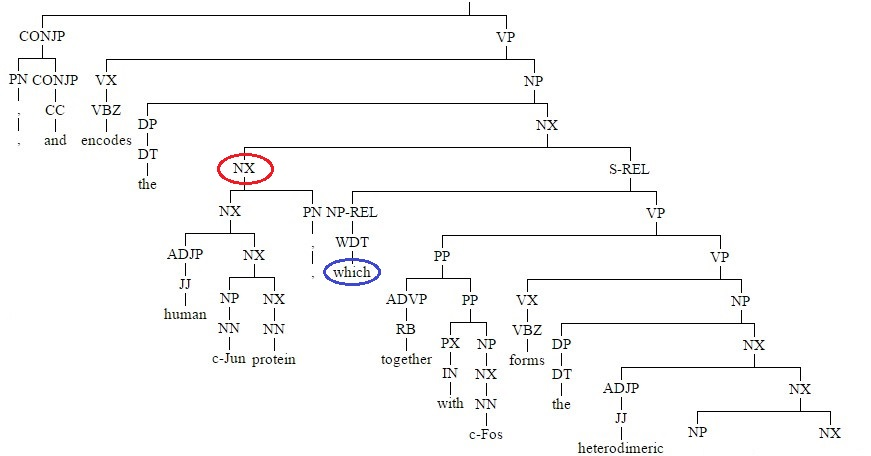
\includegraphics[scale=0.6]{relative.jpg} 
 	 \caption{ DESCRIPTION }
	 \label{Figure 11}
  \end{center}
\end{figure}
 
\subsection{Personal pronouns} 
From the statistics and mining the data set I realised that when  the personal pronoun appears in the second or third clause of the sentence then its antecedent is the  subject of the previous (nearest) clause, in the first or in the second clause, respectively.  The same rule is when in the sentence we have two coordinated noun phrases. 

If the personal pronoun appears in the first clause then the personal pronoun is the subject of the sentence. In this case, I take as antecedent the subject of the previous  sentence. I base this rules based on the assumption:\emph{"In scientific writing people try to follow the rules of cohesion and coherence. This mean that in one paragraph they do not introduce so many subjects and describe just one subject and its property."}

\begin{figure}[h]
  \begin{center}
	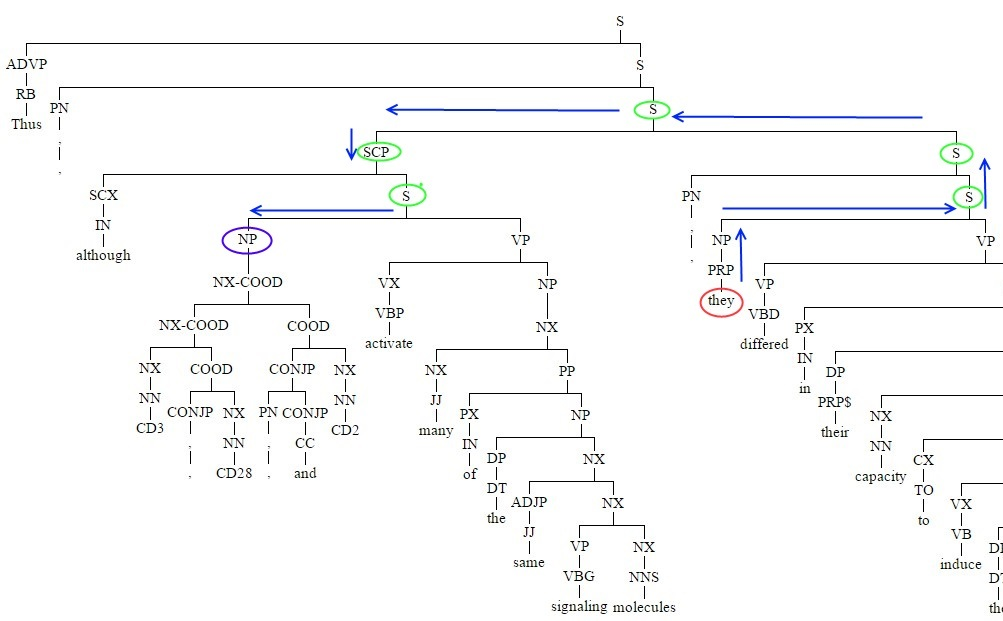
\includegraphics[scale=0.53]{PersonalPronounsNP.jpg} 
 	\caption{Simulation of  the rule when the anaphora is in the second clause and the antecedent is in the first clause of a complex sentence.}
	\label{Figure 12}
  \end{center}
\end{figure}

\footnotetext{Sentence "Thus, although CD3, CD28, and CD2 activate many of the same signaling molecules, they differed in their capacity to induce the tyrosine phosphorylation of HSI." is taken from PMID-9794375}

An exception is when we have two coordinated verb phrases. If  the anapha (it or they) appears in a coordinated verb phrase, and it is in the second verb phrase, then I do not search for antecedent in the first verb phrases because "the verb phrase describe an activity that is taken from the subject". Thus, both verb phrases of coordinated phrases describe an activity, and the activity is taken by the subject of the sentence and I select as antecedent the subject of previous clause (sentence) in which the anaphora appears. 

\begin{figure}[h]
  \begin{center}
	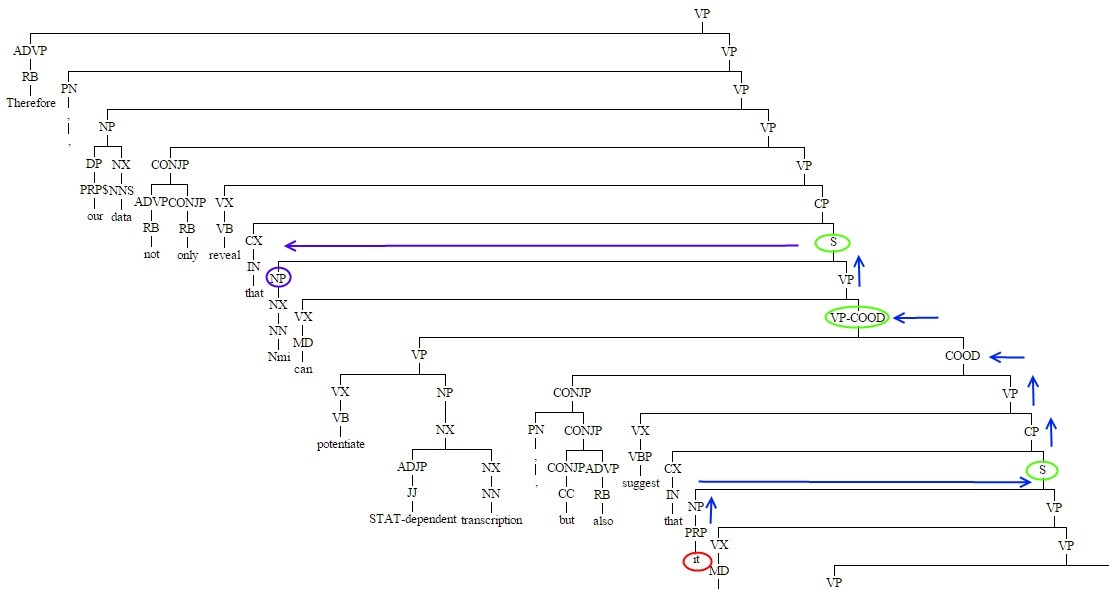
\includegraphics[scale=0.50]{PersonalPronounsVP.jpg} 
 	\caption[Caption for LOF]{Simulation of  the rule when the anaphora is in the second verb phrase of a coordinated verb phrase and I chose as antecedent the subject of the nearest clause (sentence).\footnotemark}
	\label{Figure 13}
  \end{center}
 \end{figure}
 
\footnotetext{Sentence "Therefore, our data not only reveal that Nmi can potentiate STAT-dependent transcription, but also suggest that it can augment co-activator protein recruitment to at least some members of a group of sequence-specific transcription factors." is taken from PMID-8108414}

\newpage
\subsection{Possessive pronouns}

The same idea and the same rules I applied in possessive pronouns. From the mining of the corpus,I realised that possessive pronouns appear more in coordinated noun phrases. 
\begin{figure}[h]
  \begin{center}
	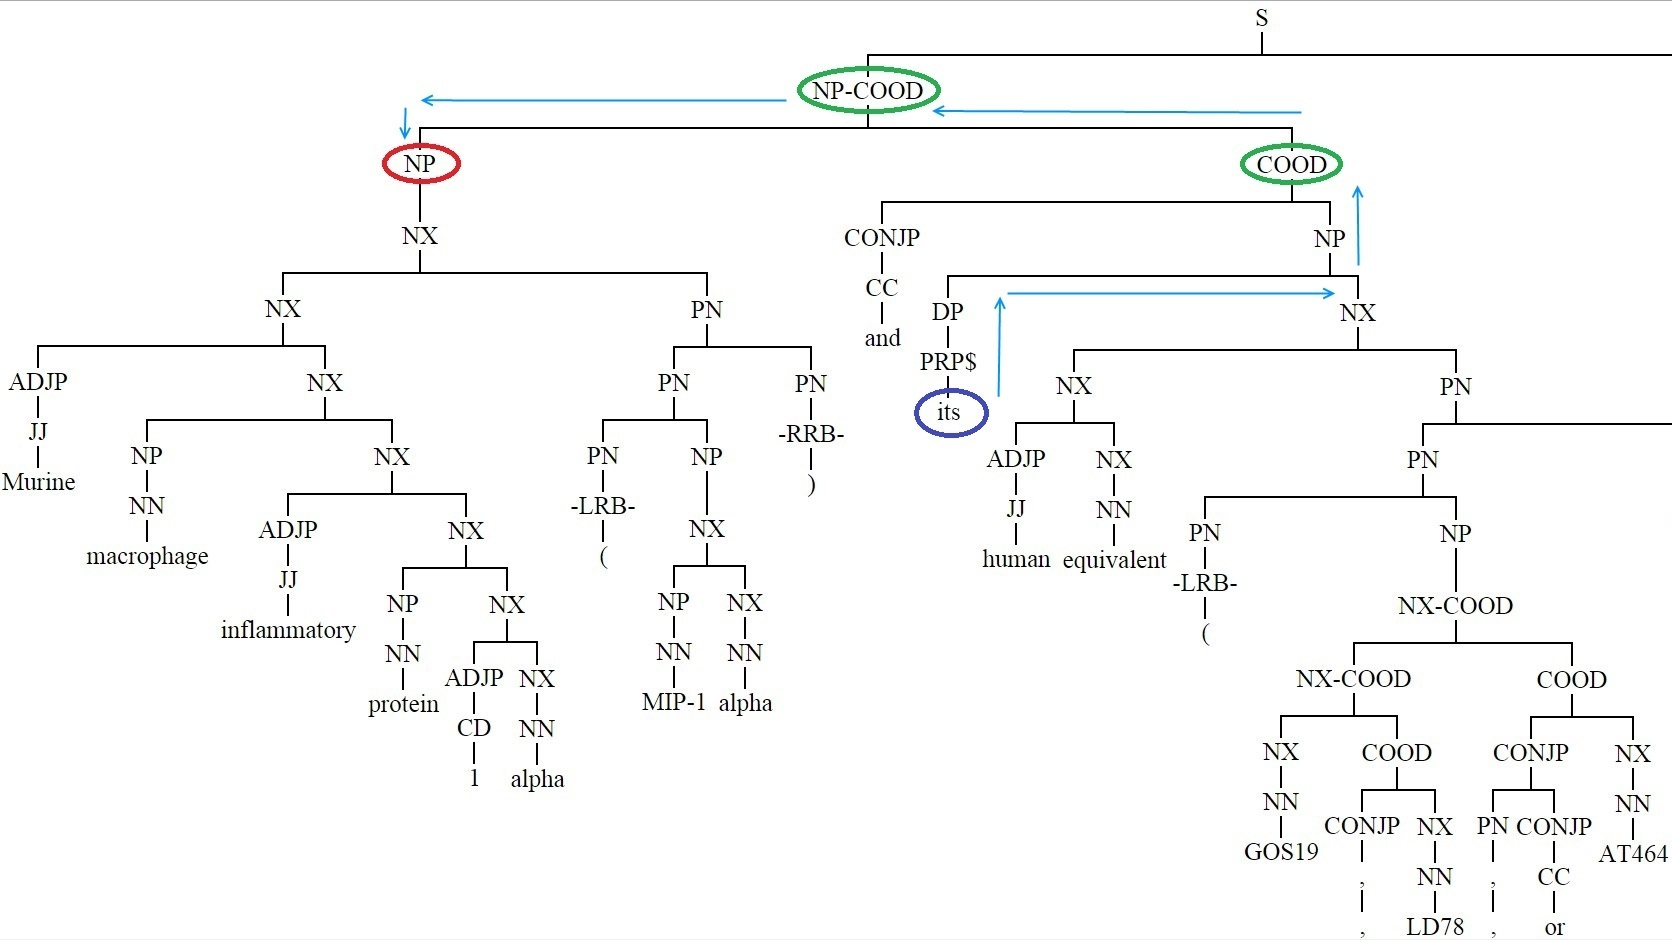
\includegraphics[scale=0.30]{PossesiveNP.jpg} 
 	\caption["to document"]{Simulation of  the rule when the anaphora  is in the second coordinated noun phrase of a coordinated noun phrase and I chose the antecedent from the previous noun phrase\footnotemark}
	\label{Figure 14}
  \end{center}
 \end{figure}
 
\footnotetext{Sentence "Therefore, our data not only reveal that Nmi can potentiate STAT-dependent transcription, but also suggest that it can augment coactivator protein recruitment to at least some members of a group of sequence-specific transcription factors." is taken from PMID-8108414}
\newpage

\begin{figure}[h]
  \begin{center}
	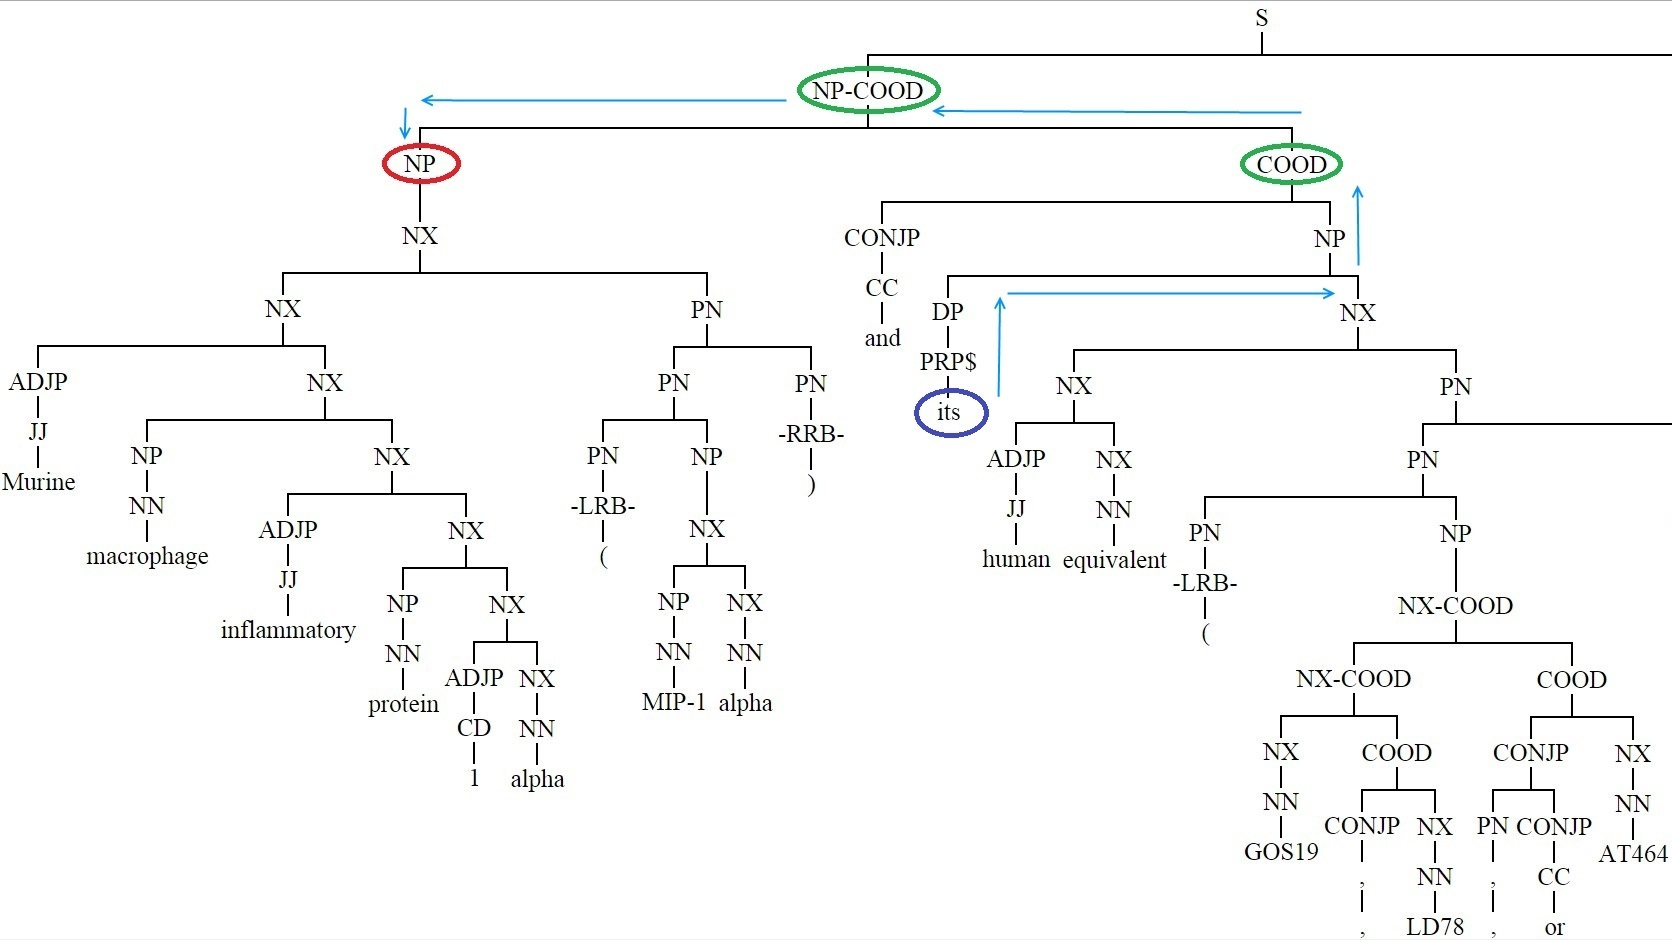
\includegraphics[scale=0.30]{PossesiveNP.jpg} 
 	\caption[Caption for LOF]{Simulation of  the rule when the anaphora  is in the second coordinated noun phrase of a coordinated noun phrase and I chose the antecedent from the previous noun phrase\footnotemark}
	\label{Figure 15}
  \end{center}
\end{figure}

\footnotetext{Sentence "Murine macrophage inflammatory protein 1 alpha (MIP-1 alpha) and its human equivalent (GOS19, LD78, or AT464) are members of the -C-C family of low-molecular-weight chemokines." is taken from PMID-7760807}

\subsection{Definite noun phrases} 

I select the nearest candidate of the candidates that fulfill the requirements of the "best" rules, then if there is no candidate selected then I run the other rules to select the nearest noun phrase that fulfill the requirements of the less accurate rules.  
